\documentclass[journal]{IEEEtran}
\usepackage[T1]{fontenc}
\usepackage{cite}
\usepackage{amsmath,amssymb}
\usepackage{booktabs,array,tabularx,multirow}
\usepackage{graphicx}
\usepackage{xcolor}
\usepackage{tikz}
\usetikzlibrary{positioning,arrows.meta,calc}
\usepackage[hidelinks]{hyperref}
\makeatletter
\setlength{\@fptop}{0pt}
\setlength{\@fpsep}{16pt plus 2pt minus 2pt}
\setlength{\@fpbot}{0pt plus 1fil}
\setlength{\@dblfptop}{0pt}
\setlength{\@dblfpsep}{16pt plus 2pt minus 2pt}
\setlength{\@dblfpbot}{0pt plus 1fil}
\makeatother
\newcolumntype{Y}{>{\raggedright\arraybackslash}X}
\newcolumntype{R}{>{\raggedleft\arraybackslash}X}
\newcommand{\I}{\mathbb{I}}
% figures/plots.py writes every figure this file includes into figures/.
\graphicspath{{figures/}}
\title{Per-account detection and refusal of task-concentrated extraction: a measurement on a model API}
\author{Rajveer~Singh, Dhruv~Deepak, Vansh~Kulshrestha, and Aryash~Kushwaha}
\begin{document}
\maketitle

\begin{abstract}
A model API hands out the supervision a competitor needs to train a copy of the model, and it does not hand it out evenly. On our bench a math answer averages 370 tokens and a news label 2.3. An attacker after a capability therefore has to collect deeply in one task, and through an account that means concentrating. Either one account works through the tasks one block at a time, or the campaign gives each task an account of its own. We built TRACE, a harness that serves a Qwen3.5-9B teacher on four tasks behind a gateway, scores each account's requests in windows of 100 with a detector built on maximum mean discrepancy, and records every released token in a ledger. We ran both collection patterns against the detector with and without memory across windows, and against a calibrated per-account quota. In both campaigns the detector singled out the math-collecting account at its first math window while every other window stayed in the benign range. It refused that account after 99 of 1,500 math answers without memory and after 199 with it. The campaigns received 6.3 to 13.3\% of the math tokens that an unprotected pass of the same prompts released. The single-account campaign also lost everything after its math block and kept 5.0 to 9.6\% of all tokens. The six-account campaign kept 35.5 to 39.9\%, and its five other accounts never left the lowest level. The quota let that campaign's math account take 1,215 math answers. In an offline replay the detector escalated 10 of 100 held-out legitimate accounts and refused 2 to 4 of them. Because the detector decides only when a window closes, the window length sets how much it releases, however strongly the account stands out. That residual is not small. Qwen3.5-2B students trained on the 95 to 197 answers released before refusal scored 70.1 to 73.5\% on 746 held-out GSM8K problems, against 51.7\% untrained, 73.5\% for a student trained on all 1,473 trainable answers and 83.0\% for the teacher. The detector stopped the release, and an earlier stop would have to act within the first window.
\end{abstract}
\begin{IEEEkeywords}
Model extraction, knowledge distillation, access control, maximum mean discrepancy, API security, measurement.
\end{IEEEkeywords}

\section{Introduction}
\IEEEPARstart{A}{nyone} who can query a model can collect its answers and train a smaller student on them~\cite{tramer2016stealing,orekondy2019knockoff,hinton2015distilling,kim2016sequence}. Providers report this at scale. Anthropic attributes more than 16 million exchanges through about 24,000 fraudulent accounts to three laboratories~\cite{anthropic2026detecting}, OpenAI reports 16,000 patterned requests from more than 4,000 users in two days~\cite{openai2026disrupting}, and Google reports one campaign of more than 100,000 prompts~\cite{gtig2026distillation}. Their defenses act on accounts. They link accounts, fingerprint behavior, verify identity, and rate-limit or ban~\cite{anthropic2026detecting,anthropic2026defenses,openai2026disrupting}.

An account-level control leaves each answer as it is. What it decides is how many answers leave before it acts, and what acting costs legitimate users. Both quantities can be read off the gateway. Published detectors report something else. They score fixed batches of queries and give a detection rate~\cite{juuti2019prada,liu2026detector,liu2026lifecycle}. A provider needs the release, meaning the responses and tokens a campaign already holds when the control refuses it, counted by task.

The task matters because distillation is aimed at a capability, and the supervision that teaches a capability is uneven. On our bench GSM8K answers average 370 tokens and carry 69\% of all released tokens, while AG News labels average 2.3. A campaign that wants a math student has to collect many math answers, and through an account that means concentrating. One account can work through the tasks in blocks, or the campaign can assign accounts to tasks. Both leave an account sending one task for hundreds of requests, and that concentration is what a per-account content score is built to see. A campaign that keeps every account evenly mixed across tasks is a different problem. Its windows look like the pooled traffic of all users, and Section~\ref{sec:scope} explains why a score of this form should not be expected to separate it. We leave that case to signals other than content.

TRACE~\cite{trace2026artifact} measures release directly. One gateway serves one teacher on four tasks. A policy layer decides per request whether to serve, slow, challenge or refuse, and a release ledger records every response that left the gateway. Scripted campaigns and simulated legitimate users share the endpoint. Figure~\ref{fig:release} shows the cumulative release of the two concentrated campaigns of run v7 under each control.

\begin{figure*}[!t]
\centering
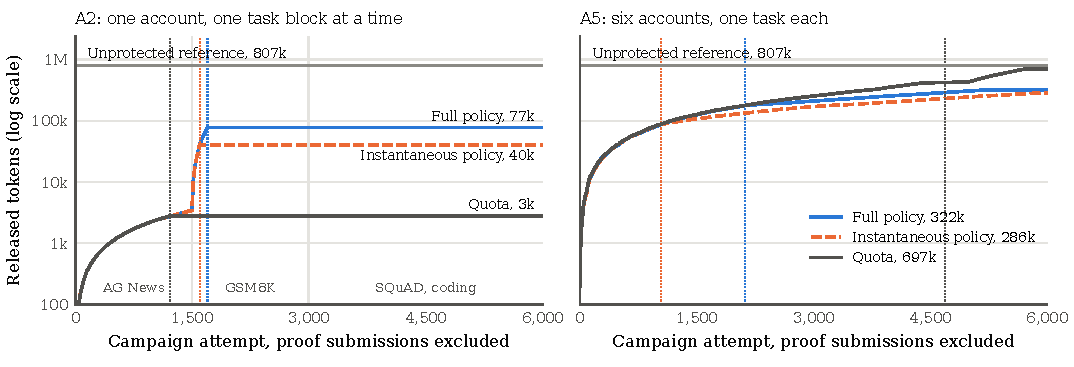
\includegraphics[width=\textwidth]{release.pdf}
\caption{Cumulative output tokens released to each campaign, from the release ledger, on a log scale. Dotted vertical lines mark each control's first refusal decision, in the color of its arm. The horizontal line is the unprotected reference, the same 6,000 prompts served with no control acting. Left: A2 sends one block per task, AG News first and GSM8K second. Both detector policies refused it inside the GSM8K block and it received nothing afterwards. The quota ran out during the AG News block. Right: A5 gives each task its own accounts. The detector refused only the GSM8K account, and the quota refused the GSM8K and SQuAD accounts once each reached 1,215 responses.}
\label{fig:release}
\end{figure*}

The detector stopped both campaigns. Our findings:
\begin{itemize}
	\item \textit{It found the account that mattered.} In both campaigns the first math window ranked 0.015 to 0.018 against benign windows, about ten times the smallest rank the calibration can produce. Every window outside the math stream ranked above 0.42 and added no risk.
	\item \textit{It stopped the release within two windows.} The instantaneous policy refused the math account after 99 answers and the full policy after 199. The campaigns kept 6.3 to 13.3\% of the math tokens an unprotected pass released.
	\item \textit{The stop held, and it was selective.} A refusal lasts until the account's horizon resets, so the single-account campaign also lost its SQuAD and coding blocks and kept 5.0 to 9.6\% of all tokens. In the six-account campaign the refusal fell on the math account alone. It still removed 60 to 65\% of the campaign's tokens, because math answers carry most of them.
	\item \textit{Content did what a count could not.} The quota held each account to 1,215 responses, so the task-dedicated math account received 1,215 math answers, 81\% of the full set. The quota denied the single-account campaign all of its math only because that campaign spent the quota on news labels first.
	\item \textit{The cost is measured.} In replay the detector escalated 10 of 100 held-out legitimate accounts under either policy. The full policy refused 4 of them and the instantaneous policy 2.
\end{itemize}

We also show that the window, not the strength of the signal, fixes when the stop arrives. A detector that scores windows of $W$ requests cannot decide anything about an account before its first window closes, so about $W$ answers in a task leave before it can act. Students trained on the release tell us whether that matters. On this bench $W=100$, and students trained on 95 and 98 released answers reached 70.8 and 73.5\% on held-out GSM8K. A student trained on all 1,473 trainable answers reached 73.5\%. What still gets out is the first window, and shrinking it is the next problem for the detector.

The evidence has limits that we state up front. It comes from one run with one seed per campaign, the exploratory half of the attacker data and synthetic legitimate users, whose concentration drives the false alarms as well as the detections. The students cover one task with one training seed each, and none trained on fewer than 95 answers.

Section~\ref{sec:related} reviews related work. Section~\ref{sec:method} describes the harness and Section~\ref{sec:scope} the collection it targets. Section~\ref{sec:protocol} gives the v7 protocol. Section~\ref{sec:detect} reports when the detector saw each campaign, Section~\ref{sec:release} what the stop withheld, and Section~\ref{sec:cost} what it cost legitimate users. Section~\ref{sec:students} sets the release against what a student learns from it, and Section~\ref{sec:discussion} discusses what an earlier stop would need.

\section{Related work}
\label{sec:related}
\textit{Extraction and distillation.} An attacker queries a victim, collects input-output pairs and trains a surrogate. Task accuracy and fidelity to the victim are different goals~\cite{jagielski2020high}. Krishna et al.\ extracted BERT-based APIs with synthetic queries, and MeaeQ picks task-relevant queries from public text~\cite{krishna2020thieves,dai2023meaeq}. Model Leeching reached 75\% exact match on SQuAD for about \$50 in API fees~\cite{birch2023leeching}, and LoRD also applies collection and training to language models~\cite{liang2025lord}. Our attacker trains on response-token cross-entropy, which is sequence-level distillation from decoded outputs~\cite{kim2016sequence}, with low-rank adapters~\cite{hu2022lora}. A student can copy a teacher's style without its capability~\cite{gudibande2024false}, so we score students on a benchmark. Extracting behavior differs from recovering training records or membership~\cite{carlini2021extracting,shokri2017membership}, and we make no privacy claim.

\textit{Per-client detection.} PRADA tracks the distribution of distances between a client's queries, and its authors note that splitting queries across clients defeats it~\cite{juuti2019prada}. Kesarwani et al.\ track feature-space coverage per user~\cite{kesarwani2018warning}, and SEAT flags near-duplicate attack queries~\cite{zhang2021seat}. VarDetect and HODA use latent query distributions and sample hardness~\cite{pal2021stateful,sadeghzadeh2022hoda}, and adaptive misinformation assumes attack queries are out of distribution~\cite{kariyappa2020adaptive}. Liu et al.\ detect extraction in language-model traffic with a kernel two-sample statistic over sentence embeddings and 1,500-query windows~\cite{liu2026detector,mmd2026artifact}. We apply their score per account with 100-request windows and add memory across windows through a decayed cumulative sum~\cite{page1954cusum}. Testing by betting and conformal test martingales make detection valid at every look under stated conditional or exchangeability assumptions~\cite{shekhar2023betting,vovk2021retrain,ramdas2023gametheoretic}. Our accumulator claims no such guarantee. Proof of work prices access in computation~\cite{dwork1992pricing}, and Dziedzic et al.\ calibrate its difficulty to how much information a user's queries reveal~\cite{dziedzic2022pow}. The proof of work in our controls has a fixed difficulty. Sun et al.\ show that stateful monitors cannot stop task decomposition across unlinkable identities without denying legitimate traffic~\cite{sun2026decomposition}. Their limit concerns identities whose traffic looks benign on its own. An account dedicated to one task does not look benign to a concentration score, which is why task-partitioned collection stays inside our target.

\textit{How much supervision a student needs.} Small sets of good answers go a long way. s1 fine-tuned a strong reasoning model on 1,000 curated examples~\cite{muennighoff2025s1}, and LIMO reports strong math reasoning from about 1\% of the data earlier work used~\cite{ye2025limo}. These results concern curated sets and stronger students than ours, but they explain why a release of a few hundred answers in one task deserves a student test.

\textit{Judging defenses.} Libon et al.\ argue that a distillation defense is only broken or unbroken relative to an attacker's query budget, data budget and interface~\cite{libon2026break}. Allouah et al.\ find that adaptive students recover much more capability than passive evaluation suggests~\cite{allouah2026game}. DistillGuard evaluates output-level defenses on a fixed 10,000-example set and excludes query detection and rate limiting~\cite{jiang2026distillguard}. A lifecycle benchmark scores ten extraction defenses, including MMD, PRADA and SEAT detectors on fixed 50-query batches~\cite{liu2026lifecycle}. None of them measures how much an account-level control releases before it acts, or what that release supports. That is the measurement this paper adds.

\textit{Output defenses.} A separate family changes what answers teach. Antidistillation sampling perturbs decoding~\cite{savani2025antidistillation}, DOGe fine-tunes the teacher's final head against a proxy~\cite{li2025doge}, lossless antidistillation sampling aims to leave the answer distribution unchanged~\cite{diao2026lossless}, and trace rewriting turns reasoning into dense formal steps~\cite{ma2026tracerewriting}. Adaptive attackers have recovered much of what such perturbations withhold~\cite{libon2026break,allouah2026game,zhu2026learnability}. Knowledge honeypots let an extractor collect planted knowledge that later exposes it~\cite{dai2026knowledgetrap}. Watermarks support an ownership claim after training~\cite{szyller2021dawn,jia2021entangled,chang2026basins}, but students can be trained to suppress the inherited signal~\cite{pan2025watermarks}. The controls we measure leave each answer unchanged and act only on access, so the two families combine.

\section{The harness}
\label{sec:method}
\subsection{Gateway and threat model}
One endpoint serves a fixed teacher across four domains, listed in Table~\ref{tab:data}. Each request carries its domain's prompt template and output cap, and the gateway rejects a request that matches no template before any policy decision. Before inference the policy layer sees the prompt, the arrival time and the authenticated account. A campaign controls one or more accounts and pools their responses into one training set. The attacker knows how the detector works and sees service actions, but not calibration data or internal scores. Bearer keys give stable identities and put no price on a new account, so one attacker can hold many identities~\cite{douceur2002sybil}. All accounts in a campaign share one budget of 6,000 HTTP attempts, 1,500 prompts per domain, within 24 hours. Failed requests and proof-of-work submissions spend attempts.

\begin{table}[!t]
\centering\footnotesize
\caption{Domains served by one gateway. Mean tokens are per released response in the unprotected reference.}
\label{tab:data}
\begin{tabularx}{\columnwidth}{@{}lYrr@{}}\toprule
Domain & Evaluation & Cap & Mean tokens \\\midrule
AG News~\cite{zhang2015char} & Topic label accuracy & 16 & 2.3 \\
SQuAD 1.1~\cite{rajpurkar2016squad} & Token F1 & 64 & 7.8 \\
GSM8K~\cite{cobbe2021gsm8k} & Numeric exact match & 1,024 & 370 \\
Coding~\cite{ahmad2025opencodeinstruct,opencodeinstructdataset,liu2023evalplus,humanevalplusdataset,mbppplusdataset} & HumanEval+ and MBPP+ pass@1 & 512 & 157 \\\bottomrule
\end{tabularx}
\end{table}

\subsection{Controls}
\label{sec:controls}
The content detector embeds each prompt with \texttt{BAAI/bge-small-en-v1.5}~\cite{xiao2024cpack,bge2023model} and scores each non-overlapping window of 100 consecutive requests from one account against 20 reference windows of pooled benign traffic with the unbiased squared MMD estimator~\cite{gretton2012kernel}. The kernel averages four RBF bandwidths around the median benign distance. Benign calibration windows give $M$ null scores $s_i^{(0)}$, and a window score $s_j$ becomes its upper-tail rank~\cite{phipson2010permutation}
\begin{equation}
p_j=\frac{1+\sum_{i=1}^{M}\I[s_i^{(0)}\geq s_j]}{M+1}.
\end{equation}
A small $p_j$ means the window is rarer than benign windows usually are. The full policy accumulates evidence with a decayed cumulative sum~\cite{page1954cusum},
\begin{equation}
r_{a,j}=\max\{0,\lambda r_{a,j-1}-\log p_{a,j}-\kappa\},\quad r_{a,0}=0,
\label{eq:risk}
\end{equation}
with $\lambda=0.9$ and $\kappa=1$, so a window adds risk only when $p_{a,j}<e^{-1}\approx0.37$. The instantaneous policy keeps no memory and uses $-\log p_{a,j}$ of the current window alone. Thresholds map risk to the levels in Table~\ref{tab:actions}, and an account keeps its highest level until its 24-hour horizon resets.

\begin{table}[!t]
\centering\footnotesize
\caption{Policy levels used in both detector arms.}
\label{tab:actions}
\begin{tabularx}{\columnwidth}{@{}lY@{}}\toprule
Level & Action \\\midrule
L0 & Serve. \\
L1 & Serve and record an alert. \\
L2 & Space admitted requests at least one second apart. \\
L3 & L2, plus a SHA-256 proof of work with 20 leading zero bits. \\
L4 & Refuse until the horizon resets. \\\bottomrule
\end{tabularx}
\end{table}

The quota is the baseline. It counts an account's requests in a horizon, serves up to its limit and refuses everything after. It reads no content.

\subsection{Ledger and cuts}
The gateway reserves each admission in a release ledger before producing output, and each reservation settles once as released, failed or cancelled. Every released-token count in this paper comes from the ledger. A checkpoint exporter cuts a campaign's ledger at each intervention, namely the first alert, the first restriction, the first refusal and the end. A cut holds exactly the responses released up to that point, never a subsample of the final ledger, so a cut is what an attacker would hold if the campaign stopped there. Figure~\ref{fig:bench} shows the path from request to cut and, for the student test of Section~\ref{sec:students}, on to a benchmark.

\begin{figure}[!t]
\centering
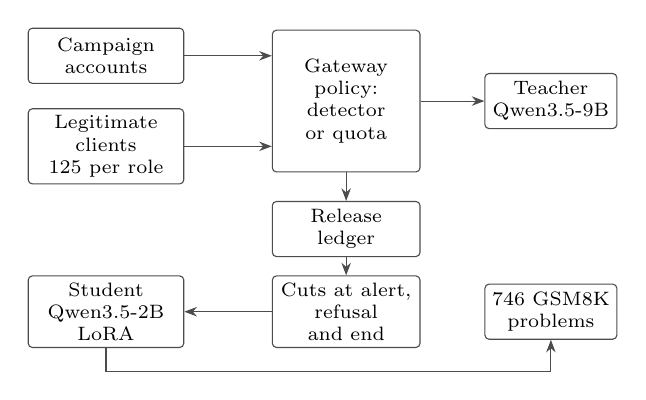
\begin{tikzpicture}[
	font=\scriptsize,
	box/.style={draw=black!70, rounded corners=1.5pt, align=center, inner sep=2.5pt, minimum height=7mm, text width=#1},
	box/.default=18mm,
	arr/.style={-{Stealth[length=1.6mm]}, draw=black!70}
]
\node[box] (atk) at (0, 0) {Campaign\\accounts};
\node[box] (ben) at (0, -1.15) {Legitimate clients\\125 per role};
\node[box=17mm, minimum height=18mm] (gw) at (3.05, -0.575) {Gateway\\policy: detector\\or quota};
\node[box=15mm] (teach) at (5.65, -0.575) {Teacher\\Qwen3.5-9B};
\node[box=17mm] (led) at (3.05, -2.2) {Release ledger};
\node[box=17mm] (cut) at (3.05, -3.25) {Cuts at alert,\\refusal and end};
\node[box] (stu) at (0, -3.25) {Student\\Qwen3.5-2B\\LoRA};
\node[box=15mm] (eval) at (5.65, -3.25) {746 GSM8K\\problems};
\draw[arr] (atk.east) -- (atk.east -| gw.west);
\draw[arr] (ben.east) -- (ben.east -| gw.west);
\draw[arr] (gw) -- (teach);
\draw[arr] (gw) -- (led);
\draw[arr] (led) -- (cut);
\draw[arr] (cut) -- (stu);
\draw[arr] (stu.south) -- ++(0,-3mm) -| (eval.south);
\end{tikzpicture}
\caption{The harness. Campaign and legitimate traffic share one gateway. The ledger records what the policy let through. Each cut is the release at one intervention, and a cut can become a training set for one student, scored on a fixed suite.}
\label{fig:bench}
\end{figure}

\subsection{Indicators}
\label{sec:indicators}
For each arm we report from the ledger the responses received, the released output tokens, and the GSM8K answers and GSM8K tokens. We give each as a share of the unprotected reference, the same 6,000 prompts served with no control acting.\footnote{The unprotected reference is the ledger of the quota arm of A6 (Table~\ref{tab:scope}), which sends the same 6,000 prompts split across six accounts at random. No account reached the quota, so no control acted and the ledger holds every response, including all 1,500 GSM8K answers. We use it as the undefended reference throughout, and the unprotected student is the student trained on it.} We count the math answers released before the first refusal of a math request, and we report the share of held-out legitimate accounts each control escalates and refuses.

For a student we report accuracy on the suite with a 95\% Wilson interval~\cite{wilson1927probable} and three ratios built from the untrained student's accuracy $a_0$, the teacher's $a_T$ and the unprotected student's $a_U$. The gain over the base is $a-a_0$. The share of the base-to-teacher gap closed is $(a-a_0)/(a_T-a_0)$. The share of the unprotected gain kept is $(a-a_0)/(a_U-a_0)$. We compare two models scored on the same items with an exact McNemar test on the items they disagree on~\cite{mcnemar1947note}, Holm-adjusted across all 21 pairs of the seven models~\cite{holm1979simple}, and with a 95\% paired bootstrap interval over items from 10,000 draws~\cite{efron1993bootstrap,koehn2004significance}.

\section{Target collection patterns}
\label{sec:scope}
Call $c$ the fraction of an account's requests that fall in one task over a stretch of its traffic. Distilling a capability needs many answers in its task. A campaign gets them through accounts in one of two ways. It can raise $c$ in time, by sending one task in a long block, or across accounts, by giving a task accounts of its own. Either way some account reaches $c$ near 1 for hundreds of requests. That is the collection TRACE's detector targets, and Table~\ref{tab:scope} names the two patterns we measure, A2 and A5.

\begin{table}[!t]
\centering\footnotesize
\caption{Collection patterns the harness implements, and what one account's window holds under each. The detector targets the first two.}
\label{tab:scope}
\begin{tabularx}{\columnwidth}{@{}lYY@{}}\toprule
ID & Accounts and order & One account's window \\\midrule
\multicolumn{3}{@{}l}{\textit{Targeted: concentrated collection}} \\
A2 & One account; one block per task, AG News first, GSM8K second. & One task for 1,500 requests at a time. \\
A5 & Six accounts, one task each: two AG News, two coding, one SQuAD, one GSM8K. & One task for the account's whole life. \\\midrule
\multicolumn{3}{@{}l}{\textit{Outside the target: mixed collection}} \\
A1 & One account; tasks interleaved. & All four tasks, close to the pooled mix. \\
A3 & One account; half the budget on in-distribution cover traffic. & Diluted by cover. \\
A4 & A1 at a lower declared request rate. & As A1; windows count requests, not time. \\
A6 & Six accounts; A1's prompts split across them at random. & A smaller copy of A1. \\
A7 & One account; A1's pattern with prompts from other corpora~\cite{greene2006bbc,trischler2017newsqa,wei2024selfcodealign}, MathQA~\cite{amini2019mathqa} for math. & All four tasks, from other sources. \\
A8 & Picks prompts from feedback during collection. & Whatever it learns to send. \\\bottomrule
\end{tabularx}
\end{table}

A1, A3, A4, A6 and A7 keep $c$ low in every account, and A8 can learn to do the same. The calibration shows why a content score of this form cannot separate them from legitimate users. Before any campaign ran, a mixture control scored 50 shuffled windows of pooled benign traffic. All 50 ranked below the median benign account window, with a median rank of 0.970. Legitimate users in this generator concentrate on one task and topic, so their windows sit away from the pooled reference, and a window that looks like the average of all users looks more ordinary than almost any single user. An account that samples every task evenly sits close to that average. Catching it needs evidence that is not in the window's content, such as links between accounts or what each account costs in output tokens. Section~\ref{sec:beyond} returns to these.

The quota has no target in this sense. It bounds each account whatever the content, and so it bounds a campaign only as far as the campaign is willing to add accounts.

\section{Protocol}
\label{sec:protocol}
\subsection{Data and users}
We split each domain's pinned source by source group into disjoint roles: development, attacker, benign fitting, score calibration, policy calibration and benign test. Code runs in fresh bubblewrap namespaces without network access~\cite{bubblewrap}. A coding candidate from the seeded OpenCodeInstruct subset qualifies only if its reference solution passes its tests there and a null stub fails them, and the builder removes duplicates and 13-gram overlap with both evaluation sources~\cite{brown2020language}. We split the attacker role again into an exploratory half for development and a confirmatory half that stays unqueried until a preregistered test. Run v7 used the exploratory half, so it is development evidence. The benign generator creates 125 synthetic accounts per role. About 10\% are generalists that use several domains and the rest are single-domain specialists that send prompts in topic-ordered blocks. Account lengths follow a Pareto distribution with shape 1.5, a 100-request minimum and a 2,000-request cap.

\subsection{Calibration}
Fitting traffic gives the reference windows and kernel bandwidth, score-calibration traffic gives the null, and policy-calibration traffic sets the thresholds so that 10, 5, 2 and 1\% of scored benign horizons reach L1 to L4. We fit the quota to the 1\% target on the same horizons. The v7 null holds 598 window scores, 199 of them from non-overlapping windows, so the smallest attainable rank is $1/599=0.0017$, and 100 scored policy horizons set the thresholds in Table~\ref{tab:cal}.

\begin{table}[!t]
\centering\footnotesize
\caption{The v7 calibration on 100 scored policy horizons. Upper bounds are Clopper-Pearson 95\%~\cite{clopper1934limits}.}
\label{tab:cal}
\begin{tabularx}{\columnwidth}{@{}Ycccc@{}}\toprule
 & L1 & L2 & L3 & L4 \\\midrule
Target rate & 0.10 & 0.05 & 0.02 & 0.01 \\
Upper bound at target & 0.164 & 0.102 & 0.062 & 0.047 \\
Full thresholds & 0.38 & 1.50 & 2.76 & 4.01 \\
Instantaneous thresholds & 1.38 & 2.24 & 3.06 & 3.50 \\
Quota, requests per horizon & & & & 1,215 \\\bottomrule
\end{tabularx}
\end{table}

\subsection{Campaigns and arms}
A2 and A5 send the same 6,000 prompts and differ only in order and account ownership. Each runs against three arms: the full policy, the instantaneous policy and the quota. Every arm gets a fresh gateway, fresh credentials and its own state. Before a detector arm sends a request, a detectability check replays the frozen campaign offline through the served calibration together with the 125 held-out benign accounts. The arm runs only if the campaign's highest level in replay is above L0 and fewer than 10\% of the benign horizons reach that level. Both A2 and A5 passed under both policies, with a replay peak of L4 for the account that collected math and L0 for every other A5 account.

The same run also included A1, A3, A6 and A7. As Section~\ref{sec:scope} predicts, none of them rose above L0 in the replay check under either policy, so their detector arms sent no traffic. Their records, quota arms included, are in the artifact~\cite{trace2026artifact}.

\subsection{Teacher, students and suite}
The teacher is \texttt{Qwen3.5-9B}~\cite{qwen2026qwen35} quantized to Q4\_K\_M, served by llama.cpp~\cite{llamacpp} on one laptop RTX~4060 in non-thinking mode at temperature 0. Every student is a LoRA adapter on \texttt{Qwen3.5-2B-Base} with rank 16, $\alpha=32$ and dropout 0.05 on all linear layers, trained for three epochs at learning rate $10^{-4}$ with an effective batch of 16, a 2,048-token limit, bf16 weights~\cite{hu2022lora,loshchilov2019adamw} and seed 42. A response enters training only if the teacher finished it, so responses stopped at the output cap are dropped. We trained five students, one on the refusal cut of each detector arm (A2 and A5 under both policies) and one on the unprotected reference. In A2 and A5 no math arrived after the refusal, so the GSM8K answers at each refusal cut are the campaign's final GSM8K answers. We trained no quota students.

We score the students and the base with greedy decoding and a 512-token limit on a frozen 746-problem GSM8K development suite, and the teacher through the same API the campaigns used. Before training any student we set 65\% as the accuracy threshold for a useful student. On 746 items a binary accuracy has a 95\% half-width of about 3.6 points near 50\%, and a paired comparison with 20\% discordant items resolves about 4.6 points at 80\% power~\cite{connor1987paired,card2020power}.

\section{Detection of the collecting account}
\label{sec:detect}
Figure~\ref{fig:ranks} shows the rank of every window both campaigns sent under the full policy. The picture is the same in each. The windows that carried math ranked 0.012 to 0.030, and every other window ranked 0.42 or higher.

\begin{figure}[!t]
\centering
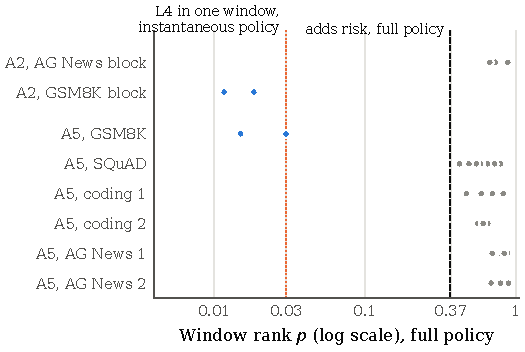
\includegraphics[width=\columnwidth]{ranks.pdf}
\caption{Window ranks of every account in A2 and A5 under the full policy, on a log scale. Windows left of the dashed line add risk under Eq.~\eqref{eq:risk}. A window left of the dotted line reaches L4 on its own under the instantaneous policy. Only the GSM8K windows, in blue, crossed either line.}
\label{fig:ranks}
\end{figure}

\subsection{A2: task blocks from one account}
A2 sent 1,500 AG News prompts first. Its fifteen AG News windows ranked between 0.65 and 0.89, so the account stayed at L0 and received every news label. The first window of its GSM8K block ranked 0.018. Under the instantaneous policy that gave a score of $-\log 0.018=4.00$, above the L4 threshold of 3.50, and the gateway refused the account at its 100th math request, after 99 answers. Under the full policy the same window gave a risk of 3.00 by Eq.~\eqref{eq:risk}. That cleared the L3 threshold of 2.76 but not the L4 threshold of 4.01, which a single window reaches only with a rank below about 0.007. The account had to solve a proof of work for its next window, which cost the campaign 100 attempts. That window ranked 0.012, the risk rose to 6.15, and the gateway refused the account at its 200th math request, after 199 answers.

\subsection{A5: one account per task}
A5's GSM8K account ranked 0.015 and 0.030 in its two windows. The other five accounts sent 43 windows between them, and the lowest ranked 0.42, so none added risk and all five stayed at L0. Under the instantaneous policy the first math window scored 4.20 and the account was refused after 99 answers. Under the full policy it reached a risk of 3.20, received a proof-of-work challenge, and was refused after its second window at a risk of 5.38, after 199 answers. Table~\ref{tab:timing} collects the timing of every arm.

\begin{table}[!t]
\centering\footnotesize
\caption{When each control acted on the campaign's math, from the release ledger. Rank and level refer to the first window of math. The attempt is the campaign attempt at the first refusal decision, proof-of-work submissions excluded.}
\label{tab:timing}
\setlength{\tabcolsep}{3pt}
\begin{tabular*}{\columnwidth}{@{\extracolsep{\fill}}llrlrr@{}}\toprule
 & Arm & Rank & Level & Math released & Attempt \\\midrule
A2 & Instantaneous & 0.018 & L4 & 99 & 1,600 \\
A2 & Full & 0.018 & L3 & 199 & 1,700 \\
A2 & Quota & & & 0 & 1,216 \\
A5 & Instantaneous & 0.015 & L4 & 99 & 1,038 \\
A5 & Full & 0.015 & L3 & 199 & 2,121 \\
A5 & Quota & & & 1,215 & 4,687 \\\bottomrule
\end{tabular*}
\end{table}

In all four detector arms the first decision on the math account came at the first moment it could. A rank exists only once a 100-request window closes, so no policy built on these windows could have refused before the 100th math request. The instantaneous policy used that first opportunity. Memory made the full policy wait one more window, because a single window has to rank below 0.007 to reach its L4 threshold alone, and a rank of 0.015 to 0.018 fell short.

\section{Release after refusal}
\label{sec:release}
Table~\ref{tab:release} gives the release of every arm, and Figure~\ref{fig:tokens} breaks it down by domain.

\begin{table}[!t]
\centering\footnotesize
\caption{Release by arm, from the ledger. Shares are of the unprotected reference, which received all 6,000 responses, 806,570 tokens, and 1,500 GSM8K answers carrying 555,498 tokens.}
\label{tab:release}
\setlength{\tabcolsep}{2.5pt}
\begin{tabularx}{\columnwidth}{@{}lrRrrrr@{}}\toprule
Arm & Served & Tokens & Share & Math & Math tokens & Share \\\midrule
A2, instantaneous & 1,599 & 40,355 & 5.0\% & 99 & 36,911 & 6.6\% \\
A2, full & 1,699 & 77,408 & 9.6\% & 199 & 73,964 & 13.3\% \\
A2, quota & 1,215 & 2,784 & 0.3\% & 0 & 0 & 0.0\% \\
A5, instantaneous & 4,599 & 286,332 & 35.5\% & 99 & 34,903 & 6.3\% \\
A5, full & 4,693 & 321,831 & 39.9\% & 199 & 71,142 & 12.8\% \\
A5, quota & 5,430 & 696,685 & 86.4\% & 1,215 & 447,418 & 80.5\% \\
Unprotected & 6,000 & 806,570 & 100\% & 1,500 & 555,498 & 100\% \\\bottomrule
\end{tabularx}
\end{table}

\begin{figure}[!t]
\centering
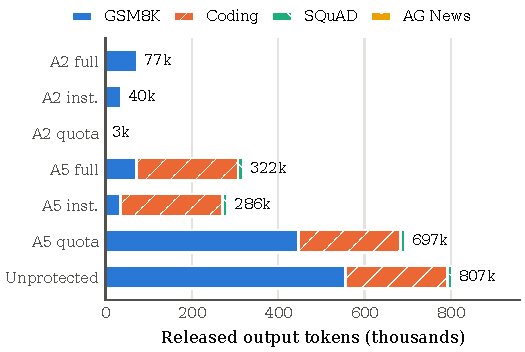
\includegraphics[width=\columnwidth]{tokens.pdf}
\caption{Released output tokens by domain for every arm of A2 and A5 and for the unprotected reference, from the release ledger. AG News and SQuAD responses are too short to show at this scale.}
\label{fig:tokens}
\end{figure}

\subsection{GSM8K release up to the first refusal}
Both detector policies held both campaigns to a small fraction of the math. The instantaneous policy released 99 of 1,500 math answers and 6.3 to 6.6\% of the math tokens. The full policy released 199 and 12.8 to 13.3\%. After the refusal no math request produced a release, and the ledger records no math for either campaign past that point.

\subsection{Persistence of refusal over the horizon}
A refused account stays at L4 until its 24-hour horizon resets, and that mattered for A2. Its SQuAD and coding blocks came after its math, from the same account, and it received none of them. A2 received its news labels, one window or two of math, and nothing else, which is 5.0\% of the unprotected tokens under the instantaneous policy and 9.6\% under the full one.

\subsection{Tokens withheld by refusing one account}
In A5 the refusal reached only the GSM8K account. The other five accounts received 4,494 responses between them under the full policy and 4,500 under the instantaneous one, including the coding answers that carry 29\% of the unprotected tokens. Even so, refusing one account in six removed 60 to 65\% of the campaign's tokens. Math answers are long, and the detector stopped the account that collected them. A control that reads content can afford to be this selective. Under the instantaneous policy it refused 1,401 of A5's requests, all from the math account, and served the other 4,599.

\subsection{Comparison with the request quota}
The quota refused every request after an account's 1,215th, so what it withheld depended on how a campaign arranged its prompts, not on what the prompts were. A2 sends news labels first, so its single account used up the quota on 1,215 labels worth 2,784 tokens and never received any math. That is the smallest release on the bench, and it came from the order of the campaign. Had A2 sent math first, the same quota would have released 1,215 math answers. A5 shows that case directly. Its GSM8K account received 1,215 math answers, 81\% of the set and 447,418 tokens, before the quota refused it, six times what the full policy let through. A count bounds an account. It cannot tell the account that matters from the others.

\section{Cost to legitimate users}
\label{sec:cost}
Table~\ref{tab:cost} gives the benign cost two ways. The offline replay asks how many held-out accounts a control escalates. Under either detector policy it was 10 of 100. Under the full policy 4 reached refusal, above the 1\% target and inside its 4.7\% upper bound, and under the instantaneous policy 2. Under the quota one held-out account of 125 sends more than 1,215 requests. It sends 1,832 and loses 617, about 2.6\% of all benign-test requests.

\begin{table}[!t]
\centering\footnotesize
\caption{Benign cost in v7. Replay uses 100 scored held-out benign horizons for the detectors and 125 held-out accounts for the quota. The live pass sent the 24,047-request benign-test schedule through each arm.}
\label{tab:cost}
\begin{tabularx}{\columnwidth}{@{}Yrrr@{}}\toprule
 & Full & Inst. & Quota \\\midrule
Replay: accounts escalated & 10 & 10 & 1 \\
Replay: reaching L1, L2, L3 & 5, 1, 0 & 5, 0, 3 & \\
Replay: refused & 4 & 2 & 1 \\
Live: benign requests refused & 464 & 0 & 0 \\
Live: served-only quality & 0.822 & 0.834 & 0.835 \\
Live: completion & 9.3\% & 11.3\% & 11.8\% \\\bottomrule
\end{tabularx}
\end{table}

The live pass measures something else, and on this hardware mostly the teacher. With a 120-second client deadline the laptop teacher completed only 9 to 12\% of requests under every arm, and about 21,300 timed out each time. Completion therefore measures teacher capacity, not policy cost. The comparable live numbers are refusals and the quality of what was served. The full policy refused 464 benign requests and the other two arms none. The quota refused nobody live because most requests timed out before admission. The utility pass ran after each campaign on separate accounts, so no run has measured a real mixture of attack and benign traffic.

The false alarms come from the same property as the detections. A legitimate specialist who works through a long block of one topic concentrates the way A2's math block does, and the score cannot tell them apart by content. Of the two policies, the instantaneous one refused fewer held-out accounts in replay, refused no live benign requests, and stopped both campaigns a window earlier.

\section{Students trained on released answers}
\label{sec:students}
A stop is worth what it withholds from the attacker's student. To place the release of Section~\ref{sec:release} in that light, we trained a student on each detector arm's refusal cut and one on the unprotected reference. Table~\ref{tab:students} reports the panel and Figure~\ref{fig:exposure} puts the students and the stops on one axis.

\begin{figure*}[!t]
\centering
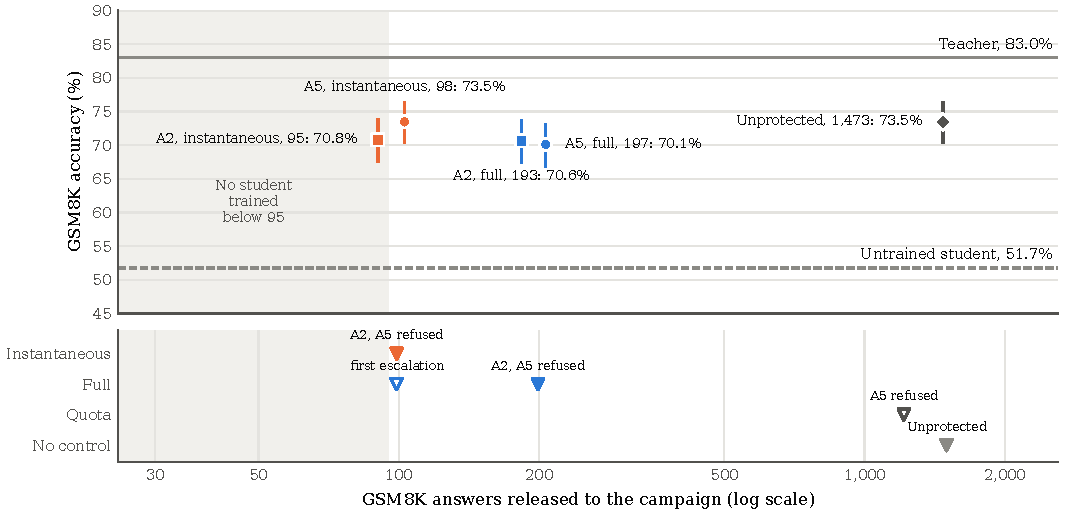
\includegraphics[width=\textwidth]{exposure.pdf}
\caption{Student accuracy and control interventions on one axis of GSM8K answers. Top: accuracy on 746 held-out problems of five students, each trained on what one arm released up to its refusal, with 95\% Wilson intervals. Students sit at their trainable count, which excludes responses stopped at the output cap. Squares mark A2 and circles A5, offset by 5\% along the axis so that they do not overlap. Bottom: GSM8K answers released before each control refused a campaign's math. Filled markers are cuts a student trained on and hollow markers are cuts with no student. The A2 quota refused before any math and cannot appear on a log axis. The shaded region, below 95 answers, holds no student.}
\label{fig:exposure}
\end{figure*}

\begin{table*}[!t]
\centering\footnotesize
\caption{The v7 GSM8K student panel on 746 development problems. Trainable answers exclude responses stopped at the output cap. Ratios are defined in Section~\ref{sec:indicators}. The last two columns compare each student with the unprotected student: a paired item-bootstrap 95\% interval and the exact McNemar $p$, with the Holm-adjusted value across all 21 model pairs in parentheses. Optimizer steps follow from the recipe as $3\lceil n/16\rceil$. The teacher row is the pass used for every comparison; two repeat passes scored 620 and 626.}
\label{tab:students}
\setlength{\tabcolsep}{3pt}
\begin{tabular*}{\textwidth}{@{\extracolsep{\fill}}lrrcrrrrcc@{}}\toprule
Model & Answers & Steps & Accuracy, \% [Wilson 95\%] & Correct & Gain, pts & Gap closed & Gain kept & Minus unprotected, pts & $p$ (Holm) \\\midrule
Untrained student & 0 & 0 & 51.7 [48.2, 55.3] & 386 & & & & & \\
A2, instantaneous & 95 & 18 & 70.8 [67.4, 73.9] & 528 & 19.0 & 61\% & 88\% & $-2.7$ [$-5.9$, $+0.5$] & 0.11 (0.55) \\
A5, instantaneous & 98 & 21 & 73.5 [70.2, 76.5] & 548 & 21.7 & 70\% & 100\% & $0.0$ [$-3.1$, $+2.9$] & 1.00 (1.00) \\
A2, full & 193 & 39 & 70.6 [67.3, 73.8] & 527 & 18.9 & 61\% & 87\% & $-2.8$ [$-5.9$, $+0.1$] & 0.082 (0.49) \\
A5, full & 197 & 39 & 70.1 [66.7, 73.3] & 523 & 18.4 & 59\% & 85\% & $-3.4$ [$-6.3$, $-0.4$] & 0.034 (0.31) \\
Unprotected & 1,473 & 279 & 73.5 [70.2, 76.5] & 548 & 21.7 & 70\% & 100\% & & \\
Teacher & & & 83.0 [80.1, 85.5] & 619 & 31.2 & & & & \\\bottomrule
\end{tabular*}
\end{table*}

\subsection{Accuracy from the first window}
Every student learned. The weakest gained 18.4 points over the untrained student and the strongest 21.7, and all five cleared the 65\% target set before training. The four students trained on what the detector released used 6.4 to 13.4\% of the unprotected run's trainable answers and closed 59 to 70\% of the gap between the base and the teacher. The unprotected student closed 70\%. Figure~\ref{fig:supervision} sets the two ratios side by side. The detector withheld 87 to 94\% of the math answers a student could train on, and the students kept 85 to 100\% of what the full set taught.

\begin{figure}[!t]
\centering
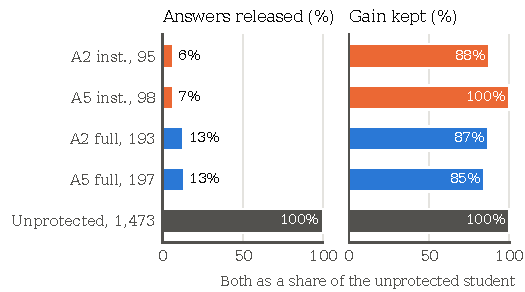
\includegraphics[width=\columnwidth]{supervision.pdf}
\caption{Left: GSM8K answers each student trained on, as a share of the unprotected run's 1,473. Right: each student's gain over the untrained student, as a share of the unprotected student's 21.7-point gain.}
\label{fig:supervision}
\end{figure}

This is the context the release figures need. The detector withheld most of the supervision, and the part it could not withhold, the first window, held most of what this recipe extracts from GSM8K answers. Withholding was large in supervision and small in capability. For the harness that turns the question from whether the detector fires, which it did in every targeted arm, into when it fires.

\subsection{Differences between students}
Figure~\ref{fig:paired} shows each student minus the unprotected one. The point estimates run from $-3.4$ to 0.0 points. Only A5 under the full policy has a raw McNemar $p$ below 0.05, 0.034 on 52 against 77 discordant items, and Holm adjustment across the panel moves it to 0.31. The 98-answer student and the 1,473-answer student solved exactly 548 problems each and disagreed on 130, split 65 and 65.

\begin{figure}[!t]
\centering
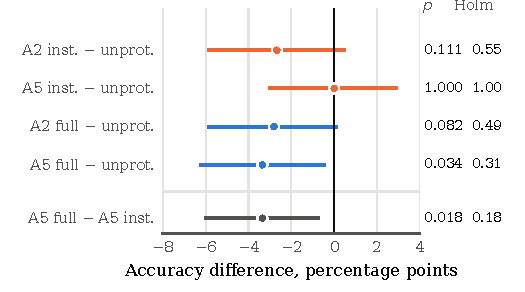
\includegraphics[width=\columnwidth]{paired.pdf}
\caption{Paired accuracy differences on the 746 problems with 95\% item-bootstrap intervals. The right columns give the exact McNemar $p$ and its Holm adjustment across all 21 model pairs. The bottom row compares two students from the same campaign.}
\label{fig:paired}
\end{figure}

The panel also shows how far one-seed students move for reasons other than data size. A5 under the instantaneous policy trained on 98 answers and beat A5 under the full policy, trained on 197, by 3.4 points (raw $p=0.018$, Holm 0.18). The student with half the data did better, by the same margin that separates the full-policy A5 student from the unprotected one. With one training seed per student, a three-point difference is within the spread this panel shows between students that differ in something other than data size.

The recipe adds a second confound. It trains for three epochs at any size, so the unprotected student took 279 optimizer steps and the instantaneous A5 student 21. More data came with more training, yet the student with a thirteenth of the steps tied the one with all of them.

\subsection{Inference variance}
We re-ran inference three times for every model on the same 746 problems. All five students and the base produced byte-identical outputs on every pass, so their scores carry no decoding noise. The teacher, served through llama.cpp, scored 619, 620 and 626, a spread of 0.9 points. We use the 619 pass throughout. Resampling by normalized question family instead of by item~\cite{field2007clustered} widens the unprotected student's interval only to 70.1 to 76.7\%.

\section{Discussion}
\label{sec:discussion}
\subsection{Window length and time to refusal}
The detector decides only when a window closes. With window length $W$ and an account that sends a fraction $c$ of its requests in one task, the earliest decision about the account comes after $W$ requests, of which about $cW$ are in that task. The detector fires on accounts with $c$ near 1, because concentration is what moves the score away from the pooled reference. So when it fires on a task, roughly $W$ answers in that task have already left, however low the window ranks. Both campaigns show this exactly. Their first math windows ranked at about ten times the calibration floor, and the instantaneous policy still released 99 answers, because that was the first moment it could decide. Memory added one more window.

On this bench $W=100$ and $c=1$ for A2's math block and A5's math account, and the students trained on 95 to 98 answers reached 70.8 and 73.5\%. To withhold the supervision that produced those students, the detector would have had to refuse at well under 100 answers. We have no student below 95, so we cannot say how far under.

Shrinking $W$ is the direct lever, and it has a price. The score of a smaller window is noisier, so its null spreads out and a legitimate specialist's block of 20 math prompts looks like an attacker's. With 100-request windows the replay already escalated 10 of 100 held-out legitimate accounts and refused up to 4. A second lever leaves $W$ alone and acts inside the first window. An account whose first 20 requests are all in one high-yield task could be slowed, not refused, until its window closes, which bounds the release at a cost to legitimate users of latency rather than service. We have measured neither.

\subsection{Mixed collection}
\label{sec:beyond}
The harness's target is the account that concentrates. Collection that keeps every account mixed, the lower half of Table~\ref{tab:scope}, needs other evidence, for the reason the mixture control gives in Section~\ref{sec:scope}. The quota does not fill that gap. It bounds what one account receives, and the ledger confirmed the bound to the request, but a campaign can add accounts until each stays under it. Sun et al.\ prove the corresponding limit for decomposition across unlinkable identities~\cite{sun2026decomposition}. Controls that act on account creation and coordination, such as linking accounts through payment or infrastructure and verifying identity~\cite{anthropic2026detecting,openai2026disrupting}, aim at that weakness. A per-account budget counted in output tokens rather than requests would at least treat a math account and a news account differently. TRACE's ledger already counts tokens per account, so such a budget can be measured the same way as the detector here, by its release, its benign cost and the student its release supports.

\subsection{Reporting release at intervention}
Released tokens and answers are what a gateway sees, and they are the right first measure of a stop. By that measure the detector did its job on both targeted campaigns. They are not the whole measure. A stop that withholds 87\% of a task's answers after the first 199 can still leave the attacker a student close to the unprotected one, as Section~\ref{sec:students} shows. We think a control aimed at distillation should report its release by task, its benign cost, and the accuracy of a student trained on the release at the cut where it intervened. TRACE produces all three from one ledger. Output defenses~\cite{savani2025antidistillation,ma2026tracerewriting} can be measured the same way, by cutting the ledger where they act and training on what went out.

\section{Limitations}
\label{sec:limits}
The release evidence is one run with one seed per campaign, on the exploratory half of the attacker data. It covers the two concentrated patterns of Table~\ref{tab:scope}, and nothing here bounds what mixed collection receives. The legitimate users are synthetic, and their topic concentration drives both the detector's false alarms and the scope argument of Section~\ref{sec:scope}. A provider whose users are mostly math tutors would see different false alarms. The utility pass ran after each campaign on a teacher that could serve only about a tenth of its requests within the deadline. Bearer keys stand in for identity, and nothing prices a new account.

The student evidence is one task, one recipe, one training seed per student and five students. The paired tests resample problems, not training runs, so they cannot see seed variance, and the panel itself suggests that variance is about three points. The recipe ties optimizer steps to data size. No student trained on fewer than 95 answers, so where useful supervision begins is unmeasured. The teacher's 83.0\% scores 96 answers that were cut at the 512-token limit as they stand, so it may understate the teacher. Coding answers, which the detector did not withhold in A5, have no student.

\section{Next steps}
\label{sec:next}
The most direct step for the detector is a smaller window, calibrated on the same benign roles, which would show what an earlier stop costs legitimate users. The early slowdown of Section~\ref{sec:discussion} is the second. The rest reuse the v7 ledgers and need no new campaign. A learning curve on random subsets of the unprotected run's GSM8K answers, at 10, 25, 50, 100, 200, 400 and 800 with several seeds each, would locate where useful supervision starts and so tell the detector how early it has to act. It would turn the shaded region of Figure~\ref{fig:exposure} into data. Two more seeds for each existing student would put an interval on training variance, and students at matched optimizer steps would separate data from training length. Finally, running A2 and A5 on the sealed confirmatory half would turn this development evidence into a test.

\section{Conclusion}
A per-account content detector can find and stop collection that concentrates on one task. On our bench it found the math-collecting account in a single-account campaign and in a six-account one, at the first math window in each, while every other window stayed in the benign range. It refused the account after 99 or 199 of 1,500 math answers, held the campaigns to 6.3 to 13.3\% of the math tokens of an unprotected pass, and never escalated the other five accounts of the six-account campaign. A request quota released six times as much math to the same account. The stop arrives when the first window closes, and students trained on what left before it kept most of what the full set taught. Shortening the time to the first refusal decision is the next step. The harness, the run records and the per-item student scores are public~\cite{trace2026artifact}.

\bibliographystyle{IEEEtran}
\bibliography{references}
\end{document}
